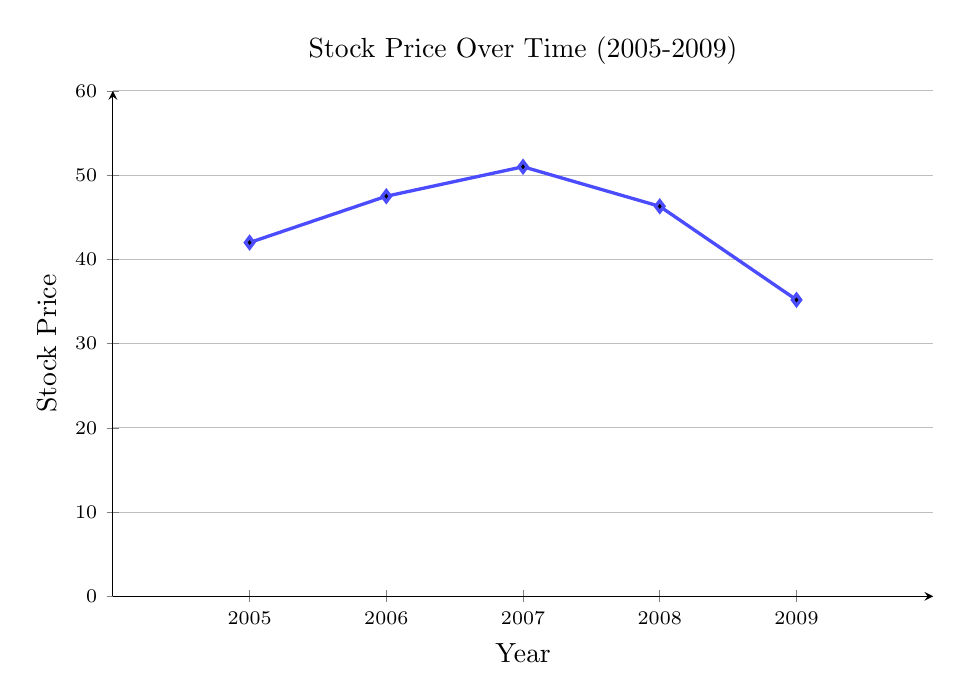
\begin{tikzpicture}[
    declare function={binom(\k,\n,\p)=\n!/(\k!*(\n-\k)!)*\p^\k*(1-\p)^(\n-\k);}
  ]
  \begin{axis}[
      axis lines=left,
      xmin = 2004, xmax=2010, ymin=0, ymax=60,
      xtick={2005,2006,2007,2008,2009},
      ytick={0,10,20,30,40,50,60}, 
      ticklabel style={font=\scriptsize},
      xticklabels={2005,2006,2007,2008,2009},
      xlabel={Year},
      ylabel={Stock Price},
      title={Stock Price Over Time (2005-2009)},
      enlargelimits=false,
      clip=false,
      grid = none,
      ymajorgrids=true,
      width=12cm,
      height=8cm
    ]
    \addplot[mark=diamond*,draw=blue!70,very thick] coordinates { 
        (2005,42)
        (2006,47.5)
        (2007,51)
        (2008,46.3)
        (2009,35.2)
    };
  \end{axis}
\end{tikzpicture}
